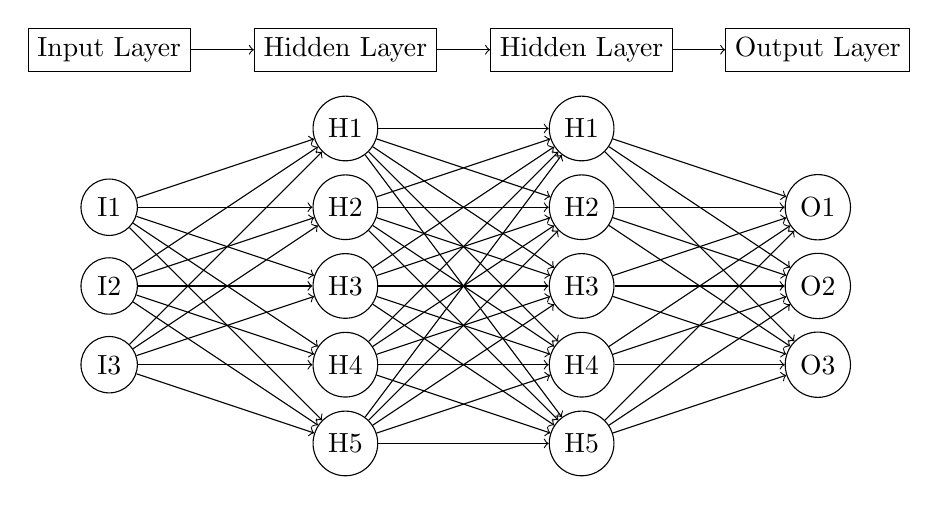
\begin{tikzpicture}
% \node at (0,6) [draw](Input Layer){Input Layer};
% \node at (3,6) [draw](Hidden Layer){Hidden Layer};

\node at (0, 3)[draw](IL){Input Layer};
\node at (3, 3)[draw](HL){Hidden Layer};
\node at (6, 3)[draw](HL2){Hidden Layer};
\node at (9, 3)[draw](OL){Output Layer};
\draw[->] (IL) -- (HL);
\draw[->] (HL) -- (HL2);
\draw[->] (HL2) -- (OL);

\foreach \y in {1,...,-1}
{
	\pgfmathtruncatemacro{\label}{2-\y};
	\node at (0, \y)[draw,shape = circle](I\label){I\label};
}

\foreach \y in {2,...,-2}
{
	\pgfmathtruncatemacro{\label}{3-\y};
	\node at (3, \y)[draw,shape = circle](H\label){H\label};
}

\foreach \y in {2,...,-2}
{
	\pgfmathtruncatemacro{\label}{3-\y};
	\node at (6, \y)[draw,shape = circle](H2\label){H\label};
}

\foreach \y in {1,...,-1}
{
	\pgfmathtruncatemacro{\label}{2-\y};
	\node at (9, \y)[draw,shape = circle](O\label){O\label};
}

\foreach \x in {1,...,3}
	\foreach \y in {1,...,5}
		\draw[->] (I\x) -- (H\y);

\foreach \x in {1,...,5}
	\foreach \y in {1,...,5}
		\draw[->] (H\x) -- (H2\y);

\foreach \x in {1,...,5}
	\foreach \y in {1,...,3}
		\draw[->] (H2\x) -- (O\y);
		


% \node at (0,2) [draw,shape = circle](I1){I1};
% \node at (0,1) [draw,shape = circle](I2){I2};
% \node at (0,0) [draw,shape = circle](I3){I3};
% \node at (3,3) [draw,shape = circle](H1){H1};
% \node at (3,2) [draw,shape = circle](H2){H2};
% \node at (3,1) [draw,shape = circle](H3){H3};
% \node at (3,0) [draw,shape = circle](H4){H4};
% \node at (3,-1) [draw,shape = circle](H5){H5};
% 


% \draw[->, color = red] (I1) -- (H1);
% \draw[->, color = red] (I1) -- (H2);
% \draw[->, color = red] (I1) -- (H3);
% \draw[->, color = red] (I1) -- (H4);
% \draw[->, color = red] (I1) -- (H5);
% \draw[->, color = red] (I2) -- (H1);
% \draw[->, color = red] (I2) -- (H2);
% \draw[->, color = red] (I2) -- (H3);
% \draw[->, color = red] (I2) -- (H4);
% \draw[->, color = red] (I2) -- (H5);
% \draw[->, color = red] (I3) -- (H1);
% \draw[->, color = red] (I3) -- (H2);
% \draw[->, color = red] (I3) -- (H3);
% \draw[->, color = red] (I3) -- (H4);
% \draw[->, color = red] (I3) -- (H5);
% 
\end{tikzpicture}
